\chapter{API Requests}

\section{HTTP Methods}

You probably already know about GET and POST requests. These are the two most commonly used requests when a web browser accesses webpages and interacts with data. All browsers, including the antiquated Internet Explorer 6 (IE6), are able to generate these two requests.

There are, however, four and a half HTTP Methods that you need to know about when building an HTTP API. I say \emph{and a half} because the PATCH method is very similar to the PUT method, and the functionality of the two are often combined into just PUT by many APIs.

You've likely heard of the phrase \emph{CRUD} when referring to the seemingly boiler-plate code many web developers need to write when interacting with a database. Some web frameworks will even generate CRUD \emph{Scaffolding} for the developer as a result of running a simple terminal command. CRUD stands for Create, Read, Update, and Delete, and short of handling any business-logic, can be used for handling all data entry.

Here is a list of HTTP Methods, as well as which CRUD operation they represent, and if your service were to represent an extremely simple database, the associated SQL command.

\begin{itemize}
\item \textbf{GET} (Read)
    \begin{itemize}
    \item Retrieve a specific Resource from the Server
    \item Retrieve a Collection of Resources from the Server
    \item Considered \emph{Safe}: this request should not alter server state
    \item Considered \emph{Idempotent}: duplicate subsequent requests should be side-effect free
    \item Corresponds to a SQL SELECT command
    \end{itemize}
\item \textbf{POST} (Create)
    \begin{itemize}
    \item Creates a new Resource on the Server
    \item Corresponds to a SQL INSERT command
    \end{itemize}
\item \textbf{PUT} (Update)
    \begin{itemize}
    \item Updates a Resource on the Server
    \item Provide the entire Resource
    \item Considered \emph{Idempotent}: duplicate subsequent requests should be side-effect free
    \item Corresponds to a SQL UPDATE command, providing null values for missing columns
    \end{itemize}
\item \textbf{PATCH} (Update)
    \begin{itemize}
    \item Updates a Resource on the Server
    \item Provide only changed attributes
    \item Corresponds to a SQL UPDATE command, specifying only columns being updated
    \end{itemize}
\item \textbf{DELETE} (Delete)
    \begin{itemize}
    \item Destroys a Resource on the Server
    \item Considered \emph{Idempotent}: duplicate subsequent requests should be side-effect free
    \item Corresponds to a SQL DELETE command
    \end{itemize}
\end{itemize}

Here are two lesser-known HTTP Methods. While it isn't always necessary that they be implemented in your API, in some situations (such as API's accessed via web browser from a different domain), their inclusion is mandatory.

\begin{itemize}
\item \textbf{HEAD}
    \begin{itemize}
    \item Retrieve metadata about a Resource (just the headers)
    \item E.g. a hash of the data or when it was last updated
    \item Considered \emph{Safe}: this request should not alter server state
    \item Considered \emph{Idempotent}: duplicate subsequent requests should be side-effect free
    \end{itemize}
\item \textbf{OPTIONS}
    \begin{itemize}
    \item Retrieve information about what the Consumer can do with the Resource
    \item Modern browsers precede all \href{http://www.w3.org/TR/cors/}{CORS} requests with an OPTIONS request
    \item Considered \emph{Safe}: this request should not alter server state
    \item Considered \emph{Idempotent}: duplicate subsequent requests should be side-effect free
    \end{itemize}
\end{itemize}

By making use of the HTTP methods, and not using actionable-verbs within the URL itself, a simpler interface is presented to the developer. Instead of wondering which verbs apply to which nouns (Do I \texttt{send} or \texttt{mail} an \emph{email}? Do I \texttt{remove} or \texttt{fire} an \emph{employee}?), a unambiguous and consistent convention is provided instead.

Typically, GET requests can be cached (and often are!) Browsers, for example, will cache GET requests (depending on expiration headers), and will go as far as alert the user if they attempt to POST data for a second time. A HEAD request is basically a GET without the response body, and can be cached as well.

If you plan on allowing JavaScript Consumers running within web browsers, and making requests from different domains, the OPTIONS method will need to be supported. There is a fairly-new concept called \href{https://en.wikipedia.org/wiki/Cross-origin_resource_sharing}{Cross Origin Resource Sharing (CORS)} which uses the OPTIONS header. Basically, it provides a set of request and response headers for defining which domains can access data and which HTTP Methods they can utilize.


\section{URL Endpoints}

An Endpoint is a URL within your API which provides a method to interact with a Resource or a Collection of Resources. A typical HTTP API will use a plural naming convention for Collections.

\subsection{Top-Level Collections}

\begin{figure}[ht!]
\centering
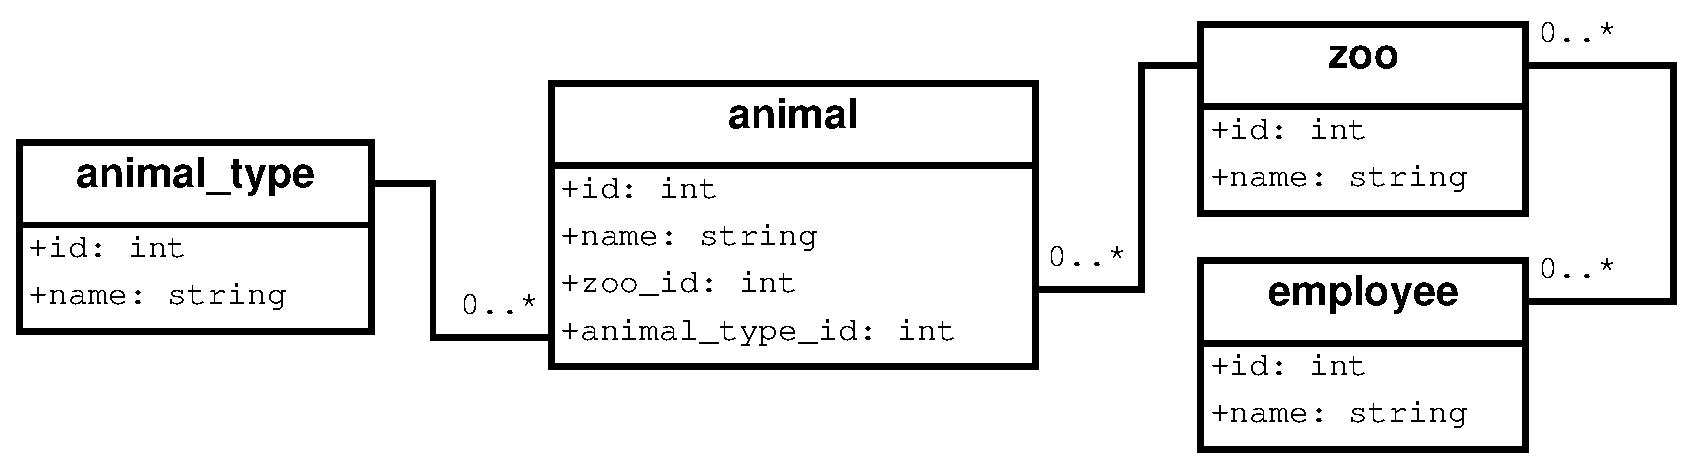
\includegraphics[width=12cm]{images/zoo-relationships.eps}
\caption{Diagram of Relationships}
\label{fig:zoorelationships}
\end{figure}

If you were building a fictional API to represent several different Zoo's, each containing many Animals (with an animal belonging to exactly one Zoo), employees (who can work at multiple Zoos) and keeping track of the species of each animal, you might have the following endpoints:

\begin{itemize}
\item \texttt{https://api.example.com/v1/\textbf{zoos}}
\item \texttt{https://api.example.com/v1/\textbf{animals}}
\item \texttt{https://api.example.com/v1/\textbf{animal\_types}}
\item \texttt{https://api.example.com/v1/\textbf{employees}}
\end{itemize}

Each piece of data separated by a slash is a URL Segment. Try to keep the number of segments per endpoint as few as possible.

\subsection{Specific Endpoints}

While conveying what each endpoint does, you'll want to list valid HTTP Method and Endpoint combinations. For example, here's a list of actions one can perform with our fictional Zoo-keeping API. Notice that we precede each endpoint with the HTTP Method. This is a common notation and is similar to the one used within an HTTP Request header.

\begin{itemize}
\item \texttt{GET /v1/zoos}: List all Zoos (perhaps just ID and Name, not too much detail)
\item \texttt{POST /v1/zoos}: Create a new Zoo
\item \texttt{GET /v1/zoos/\{zoo\_id\}}: Retrieve an entire Zoo resource
\item \texttt{PUT /v1/zoos/\{zoo\_id\}}: Update a Zoo (entire resource)
\item \texttt{PATCH /v1/zoos/\{zoo\_id\}}: Update a Zoo (partial resource)
\item \texttt{DELETE /v1/zoos/\{zoo\_id\}}: Delete a Zoo
\item \texttt{GET /v1/zoos/\{zoo\_id\}/animals}: Retrieve a listing of Animals (ID and Name)
\item \texttt{GET /v1/animals}: List all Animals (ID and Name)
\item \texttt{POST /v1/animals}: Create a new Animal
\item \texttt{GET /v1/animals/\{animal\_id\}}: Retrieve an Animal resource
\item \texttt{PUT /v1/animals/\{animal\_id\}}: Update an Animal (entire resource)
\item \texttt{PATCH /v1/animals/\{animal\_id\}}: Update an Animal (partial resource)
\item \texttt{GET /v1/animal\_types}: Retrieve a listing (ID and Name) of all Animal Types
\item \texttt{GET /v1/animal\_types/\{animaltype\_id\}}: Retrieve an entire Animal Type resource
\item \texttt{GET /v1/employees}: Retrieve an entire list of Employees
\item \texttt{GET /v1/employees/\{employee\_id\}}: Retrieve a specific Employee
\item \texttt{GET /v1/zoos/\{zoo\_id\}/employees}: Retrieve a listing of Employees at this Zoo
\item \texttt{POST /v1/employees}: Create a new Employee
\item \texttt{POST /v1/zoos/\{zoo\_id\}/employees}: Hire an Employee at a specific Zoo
\item \texttt{DELETE /v1/zoos/\{zoo\_id\}/employees/\{employee\_id\}}: Fire an Employee from a Zoo
\end{itemize}

The Entrypoint prefix has been omitted in the above examples for brevity. While this can be fine during informal communication (or books with limited page width), in your actual API documentation you should display the full URL to each endpoint.

Notice how the relationships between data is conveyed, for example the many-to-many relationships between Employees and Zoos. By adding an additional URL segment, one can perform relationship interactions. Of course there is no HTTP verb for "FIRE"-ing an employee, but by performing a DELETE on an Employee located within a Zoo, we're able to achieve the same goal.

Also notice how the listing of Endpoints doesn't include every possible method-to-resource combination. For example a Consumer is unable to POST or DELETE to the \texttt{animal\_types} Endpoints. In this fictional situation, only administrators would be able to add new \texttt{animal\_types} using some mechanism outside of the API.

There's nothing wrong with not supporting every method-to-resource combination, as every conceptual data manipulation your service offers doesn't necessarily need to be exposed via API. Just keep in mind developers may wonder why certain features aren't available, and they may even attempt to use an undocumented Endpoint (such as DELETE-ing an \texttt{animal\_type}). Know that if the functionality isn't documented, a developer may still discover a hidden feature by brute force.


\section{Filtering Resources}

When a Consumer makes a GET request for a Collection, provide them a list of every Resource matching the requested criteria, even though the list could be quite large. Do your best to minimize arbitrary limitations imposed on Consumers, as these limits make it harder for a third party developer to grok the API. If they request a Collection, and iterate over the results, never seeing more than 100 items, it is now their mission to determine where this limit is imposed. Is their ORM buggy and limiting items to 100? Is the network chopping up large responses?

Do offer the ability for a Consumer to specify some sort of filtering/limitation of the results. The most important reason for this, as far as the Consumer is concerned, is that the network payload is minimal and the Consumer receives results as soon as possible. Another reason for this is the Consumer may be lazy and want the Server to perform filtering and pagination. The not-so-important reason from the Consumers perspective, yet a great benefit for the Server, is that response-generation will require less resources.

Since these are GET requests on Collections, filters should be passed via URL parameters. Here are some examples of the types of filtering you could conceivably add to your API, and if your API were a simple representation of a Relational Database, the correlating SQL clause.

\begin{itemize}
\item \texttt{?limit=10\&offset=20}: Pagination and offsetting of results\newline{}(\texttt{LIMIT 20, 10})
\item \texttt{?animal\_type\_id=1}: Filter records which match the following condition\newline{}(\texttt{WHERE animal\_type\_id = 1})
\item \texttt{?sort\_attribute=name,asc}: Sort the results based on the specified attributes\newline{}(\texttt{ORDER BY name ASC})
\end{itemize}

Some filtering can be redundant with other endpoints. In the Endpoints section we had a \texttt{GET /zoo/\{zoo\_id\}/animals} Endpoint. This would be the same thing as \texttt{GET /animals?zoo\_id=\{zoo\_id\}}. Dedicated endpoints will make API consumption easier for developers. This is especially true with requests you anticipate will be made frequently. In the documentation, mention this redundancy so that developers aren't left wondering what the differences is.


\section{White-Listing Attributes}

Often times, when a Consumer is making a GET request to a specific Resource or Collection, they do not need all attributes belonging to the resource(s). Having so much data could become a network bottleneck as well. Responding with less data can help reduce server overhead, e.g. it may prevent an unnecessary database \texttt{JOIN}.

Again, since we're dealing with GET requests, you'll want to accept a URL parameter for white-listing attributes. In theory, black-listing could work as well, but as new attributes appear in Resources (since additions are backwards compatible), the Consumer ends up receiving data it doesn't want.

The parameter name you choose isn't too important. It could be \texttt{filter} or the overly-verbose \texttt{attribute\_whitelist}. Consistency between different Endpoints is what is most important.

The SQL queries in these examples are over-simplification of what could be generated if your API represented a simple Relational Database application.

\subsection{Filtered Request}

In this example, the Consumer has requested a filtered list of attributes pertaining to a user.

\paragraph{\textbf{Request URL}}

\begin{verbatim}
GET http://api.example.org/user/12?whitelist=id,name,email
\end{verbatim}

\paragraph{\textbf{Resulting SQL Query}}

\begin{verbatim}
SELECT id, name, email FROM user WHERE user.id = 12;
\end{verbatim}

\paragraph{\textbf{Response Body}}

\begin{verbatim}
{
  "id": "12",
  "name": "Thomas Hunter II",
  "email": "me@thomashunter.name"
}
\end{verbatim}

\subsection{Unfiltered Request}

In this example request, the default representation of a user resource includes data from two database tables joined together. One of the tables is a \texttt{user} table, and another table contains some textual data related to a user called \texttt{user\_desc}.

\paragraph{\textbf{Request URL}}

\begin{verbatim}
GET http://api.example.org/user/12
\end{verbatim}

\paragraph{\textbf{Resulting SQL Query}}

\begin{verbatim}
SELECT * FROM user LEFT JOIN user_desc ON user.id = user_desc.id WHERE user.id = 12;
\end{verbatim}

\paragraph{\textbf{Response Body}}

\begin{verbatim}
{
  "id": "12",
  "name": "Thomas Hunter II",
  "age": 27,
  "email": "me@thomashunter.name",
  "description": "Blah blah blah blah blah."
}
\end{verbatim}


\section{Body Formats}

A common method for APIs to receive data from third-parties is to accept a JSON document as the body. Assuming your API provides data to third-parties in the form of JSON, as a consequence those same third-parties should also be able to produce JSON documents.

There are two primary methods a Web Browser will use when sending data to a web server. If you're using a popular web language/framework for building an API, such as \emph{PHP} or \emph{Express.js} and \emph{Ruby on Rails}, you're already used to consuming data using these two methods. Web Servers (e.g. \emph{Apache} or \emph{NGINX}) abstract the differences of these two methods and will provide your programming language one easy method to consume data. The two methods are called Multi-part Form Data (required for file uploads), and URL Form Encoded (most forms use this latter method).

\subsection{JSON}

The JSON document used for the Request can be very similar to the JSON document used for the Response. JSON can specify the type of data (e.g. Integers, Strings, Booleans), while also allowing for hierarchal relationships of data. String data needs to be escaped (e.g. a quote \texttt{"} becomes prefixed with a backslash \texttt{\symbol{92}"}), but this is typically done automatically for the developer.

\begin{verbatim}
POST /v1/animal HTTP/1.1
Host: api.example.org
Accept: application/json
Content-Type: application/json
Content-Length: 24

{
  "name": "Gir",
  "animal_type": "12"
}
\end{verbatim}

\subsection{Form URL Encoded}

This method is used by Websites for accepting simple data forms from a web browser. Data needs to be URL Encoded if it contains any special characters (e.g. a space character becomes \texttt{\%20}). This is automatically taken care of by the browser.

\begin{verbatim}
POST /login HTTP/1.1
Host: example.com
Content-Length: 31
Accept: text/html
Content-Type: application/x-www-form-urlencoded

username=root&password=Zion0101
\end{verbatim}

\subsection{Multi-Part Form Data}

This method is used by Websites for accepting more complex data from a web browser, such as file uploads. No escaping needs to happen, although the boundary is a random string and needs to not be contained within the uploaded file or form data.

\begin{verbatim}
POST /file_upload HTTP/1.1
Host: example.com
Content-Length: 275
Accept: text/html
Content-Type: multipart/form-data; boundary=----RANDOM_jDMUxq4Ot5

------RANDOM_jDMUxq4Ot5
Content-Disposition: form-data; name="file"; filename="hello.txt"
Content-Type: application/octet-stream

Hello World
------RANDOM_jDMUxq4Ot5
Content-Disposition: form-data; name="some_checkbox"

on
------RANDOM_jDMUxq4Ot5--
\end{verbatim}
